\begin{tikzpicture}[remember picture,overlay]
    \node[xshift=-0.9in,yshift=-0.9in,anchor=north east] at (current page.north east){%
    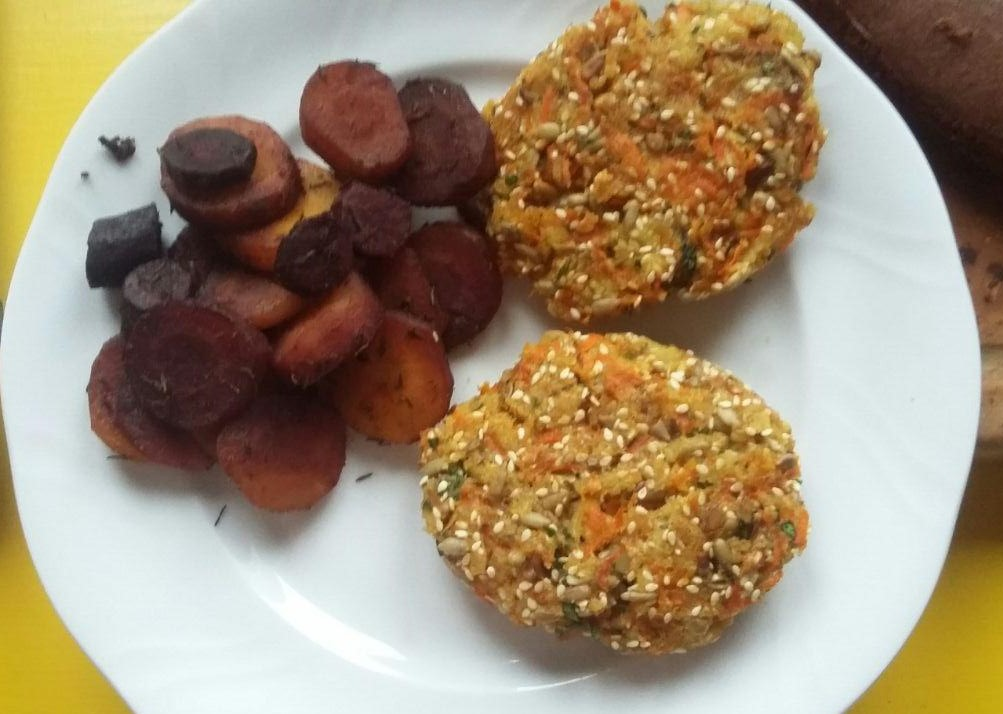
\includegraphics[width=6cm]{pic/vegeburgers}};
\end{tikzpicture}


\begin{recipe}
    [% 
        preparationtime = {\unit[30]{min}},
        bakingtime = {\unit[30]{min}}
    ]
    {Best wege patty \\
    Polish edition}
    % TODO: fix indentation
   \prerecipeoverview{
       \vspace{5mm}
   } 
    \setRecipeLengths{
        ingredientswidth=6cm
    }
    \ingredients[12]{%
        2 c. & Grated carrot \\
        0.75 c. & Millet \\
        \nicefrac{1}{2} c. & Roast sunflower seed \\
        \nicefrac{1}{2} c. & Roast sesame \\
        1 & Red onion \\
        \nicefrac{1}{2} c. & Breadcrumbs \\
        \nicefrac{1}{4} c. & Oil \\
        3 tbs. & Flour \\
        4 tbs. & Soy sauce \\
        2 ts. & Coriander powder \\
        \nicefrac{1}{2} bunch & Parsley \\
        1 ts. & Ginger \\
        & Chili \\
        &Sat\&pepper
    }

    \preparation{%
        \step Cook millet: rinse with water, rinse well with boiling water, cook in 2.25 c.
        of hot salted water, covered, for 12-15 min.
        Don't stir.
        \step Dice onion and chop parsley.
        Mix all ingredients.
        \step If the mixture is not gluey enough, add more oil/flour.
        \step Form patties and put on baking paper.
        \step Bake at \unit[200]{\textcelcius} for 30 min, turn patties after 15 min.
        \vspace{3cm}
    }

    \suggestion
    {%
        Serve either as burgers, or as main dish with roast vegetables.
        Mango chutney, good (why not home-made?) ketchup or garlic dip go well with patties.
    }
    \hint{%
        Watch out, it's very easy to burn sesame when roasting!
    }

\end{recipe}
